\section{Package Model}\begin{figure}[h!]
\begin{center}
	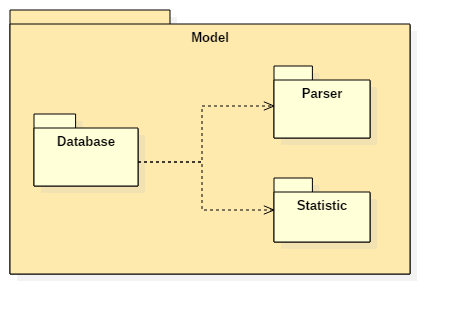
\includegraphics[scale=0.7]{../images/ModelPackage.png}
\end{center}
\end{figure}
\subsection{Model::Database}
\subsubsection{Model::Database::Database}
\begin{itemize}
\item\textbf{Funzione}:
\item\textbf{Relazioni con altre componenti}\\
La classe utilizza:
	\begin{itemize}
		\item
	\end{itemize}
\item\textbf{Attributi}:
	\begin{itemize}
		\item\code{}\\
		\item\code{}\\
		\item\code{}\\
		\item\code{}\\
	\end{itemize}
\item\textbf{Metodi}:
	\begin{itemize}
		\item\code{}\\
		\textbf{Parametri}:
			\begin{itemize}
				\item\code{}\\
			\end{itemize}
		\item\code{}\\
		\textbf{Parametri}:
			\begin{itemize}
				\item\code{}\\
			\end{itemize}
		\item\code{}\\
		\textbf{Parametri}:
			\begin{itemize}
				\item\code{}\\
			\end{itemize}
		\item\code{}\\
		\textbf{Parametri}:
			\begin{itemize}
				\item\code{}\\
			\end{itemize}
	\end{itemize}
\end{itemize}

\subsection{Model::Parser}
\subsubsection{Model::Parser::Parser}
\begin{itemize}
\item\textbf{Funzione}:
\item\textbf{Relazioni con altre componenti}\\
La classe utilizza:
	\begin{itemize}
		\item
	\end{itemize}
\item\textbf{Attributi}:
	\begin{itemize}
		\item\code{}\\
		\item\code{}\\
		\item\code{}\\
		\item\code{}\\
	\end{itemize}
\item\textbf{Metodi}:
	\begin{itemize}
		\item\code{}\\
		\textbf{Parametri}:
			\begin{itemize}
				\item\code{}\\
			\end{itemize}
		\item\code{}\\
		\textbf{Parametri}:
			\begin{itemize}
				\item\code{}\\
			\end{itemize}
		\item\code{}\\
		\textbf{Parametri}:
			\begin{itemize}
				\item\code{}\\
			\end{itemize}
		\item\code{}\\
		\textbf{Parametri}:
			\begin{itemize}
				\item\code{}\\
			\end{itemize}
	\end{itemize}
\end{itemize}

\subsection{Model::Statistics}
\subsubsection{Model::Statistics::Statistics}
\begin{itemize}
\item\textbf{Funzione}:
\item\textbf{Relazioni con altre componenti}\\
La classe utilizza:
	\begin{itemize}
		\item
	\end{itemize}
\item\textbf{Attributi}:
	\begin{itemize}
		\item\code{}\\
		\item\code{}\\
		\item\code{}\\
		\item\code{}\\
	\end{itemize}
\item\textbf{Metodi}:
	\begin{itemize}
		\item\code{}\\
		\textbf{Parametri}:
			\begin{itemize}
				\item\code{}\\
			\end{itemize}
		\item\code{}\\
		\textbf{Parametri}:
			\begin{itemize}
				\item\code{}\\
			\end{itemize}
		\item\code{}\\
		\textbf{Parametri}:
			\begin{itemize}
				\item\code{}\\
			\end{itemize}
		\item\code{}\\
		\textbf{Parametri}:
			\begin{itemize}
				\item\code{}\\
			\end{itemize}
	\end{itemize}
\end{itemize}